\begin{frame}{Semana 1 (06/02/2024) - T1}
        \textbf{Trabajo}

        $$W_{12}=\int_{1}^{2}\vec{\boldsymbol{F}}\boldsymbol{\cdot} d\vec{\boldsymbol{s}}.$$
\end{frame}

\begin{frame}{Semana 1 (06/02/2024) - T1P1}

La masa del niño es $m$, la longitud
de las cadenas es $R$, y se empuja con una fuerza $F$ hasta que las cadenas forman un
ángulo $\theta_0$ con la vertical. La fuerza $F$ es horizontal, variable, comienza en cero y aumenta en forma gradual apenas lo suficiente para que el niño y el columpio se muevan lentamente y permanezcan casi en equilibrio.

¿Qué trabajo total realizan todas las
fuerzas sobre el niño? ¿Qué trabajo realiza la tensión en las cadenas? ¿Qué trabajo efectúa la fuerza $F$? (Ignore el peso
de las cadenas y el asiento).

\begin{figure}[H]
    \centering
    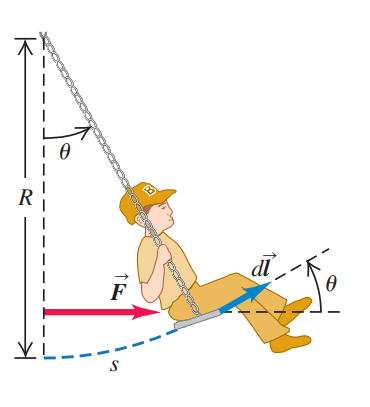
\includegraphics[width=0.3\textwidth]{figures/t1t1.png}
\end{figure}
    
\end{frame}

\begin{frame}{Semana 1 (06/02/2024) - T1}
    \textbf{Energía cinética}
    $$W_{12}=K_2-K_1=\frac{m}{2}\left(v_2^2-v_1^2\right).$$
    
    \textbf{Energía potencial}
    
    Si $W_{12}$ es independiente de la trayectoria:
    $$W_{12}=U_1-U_2,$$
    $$\vec{\boldsymbol{F}}=-\vec{\boldsymbol{\nabla}}U(\vec{\boldsymbol{r}}),$$
    $$\oint_1^2\vec{\boldsymbol{F}}\boldsymbol{\cdot} d\vec{\boldsymbol{s}}=0.$$
    
    \textbf{Conservación de la energía}
    $$K_1+U_1=K_2+U_2.$$
\end{frame}

\begin{frame}{Semana 1 (06/02/2024) - T1P2}

    \textbf{Atwood's Machine}

    \begin{figure}[H]
    \centering
    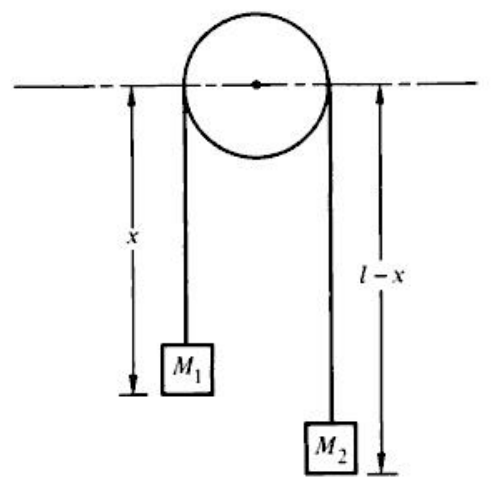
\includegraphics[width=0.5\textwidth]{figures/t1t2.png}
\end{figure}
    
\end{frame}

\begin{frame}{Semana 2 (13/02/2024) - T2P1}
        $X$ e $Y$ son dos esferas de metal sin carga sobre soportes aislantes y están en contacto entre sí. Una barra R cargada positivamente se acerca a $X$ como se muestra en la figura (a).
        
        La esfera $Y$ ahora se aleja de $X$, como en la figura (b).
        
        ¿Cuáles son los estados de carga finales de $X$ e $Y$?
        
        \begin{figure}
            \centering
            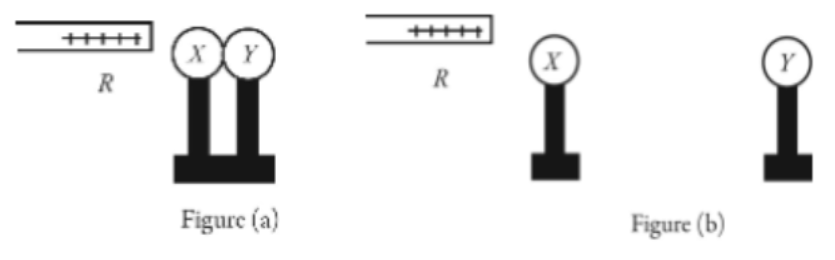
\includegraphics[scale=0.3]{figures/t2p1.png}
        \end{figure}
        
        \begin{columns}
        \column{0.5\textwidth}
        \begin{itemize}
            \item[A)] Tanto $X$ como $Y$ son neutros.
            \item[B)] $X$ es positivo e $Y$ es neutro.
            \item[C)] $X$ es neutro e $Y$ es positivo.
            \end{itemize}
        \column{0.5\textwidth}
        \begin{itemize}
            \item[D)] $X$ es negativo y $Y$ es positivo.
            \item[E)] Tanto $X$ como $Y$ son negativos.
        \end{itemize}
        \end{columns}
        
        
        
        \pause\bigskip\centering \textbf{Respuesta:} D.
\end{frame}

\begin{frame}{Semana 2 (13/02/2024) - T2P2}
    
    Una carga puntual positiva $Q$ está fija sobre una mesa horizontal muy grande sin fricción. Una segunda carga puntual positiva $q$ se libera desde el reposo cerca de la carga estacionaria y puede moverse libremente. ¿Qué enunciado describe mejor el movimiento de $q$ después de que se suelta?
    
    \begin{itemize}
    
    \item[A)]Su velocidad será máxima justo después de que se suelte.

    \item[B)] Su aceleración es cero justo después de que se suelta.
    
    \item[C)] A medida que se aleja más y más de $Q$, su aceleración seguirá aumentando.
    
    \item[D)] A medida que se aleja más y más de $Q$, su velocidad disminuirá.
    
    \item[E)] A medida que se aleja más y más de $Q$, su velocidad seguirá aumentando.
    \end{itemize}
    
    \pause\bigskip\centering\textbf{Respuesta:} E.
    
\end{frame}

\begin{frame}{Semana 2 (13/02/2024) - T2P3}
    
    Una bola de plástico muy pequeña cargada uniformemente está ubicada directamente encima de otra carga similar en un tubo de ensayo como se muestra en la figura. Las bolas están en equilibrio a una distancia $d$.
    
    \begin{columns}
    \column{0.5\textwidth}
     \begin{figure}
        \centering
        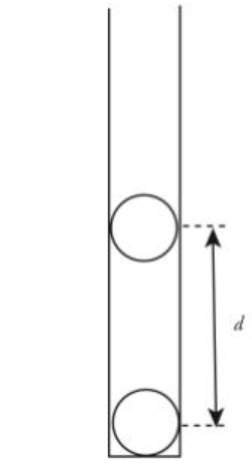
\includegraphics[scale=0.3]{figures/t2p3.png}
    \end{figure}
    
    \column{0.5\textwidth}

Si se duplica la carga de cada bola, la distancia entre las bolas en el tubo de ensayo sería
    
     \begin{itemize}
        \item[A)] $\sqrt{2}d$
        \item[B)] $2d$
        \item[C)] $4d$
        \item[D)] $8d$
    \end{itemize}
    
    \pause\bigskip\centering\textbf{Respuesta:} B.

    \end{columns}
    
\end{frame}

\begin{frame}{Semana 2 (13/02/2024) - T2P4}
    
    En la figura, $Q = 5.8$ nC. ¿Cuál es la magnitud de la fuerza el\'ectrica sobre la carga $Q$?
    
    \begin{figure}
        \centering
        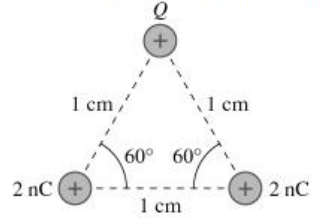
\includegraphics[scale=0.5]{figures/t2p4.png}
    \end{figure}
    
\end{frame}

\begin{frame}{Semana 2 (13/02/2024) - T2P5}
    Cuatro cargas puntuales negativas iguales están ubicadas en las esquinas de un cuadrado, sus posiciones en el plano $xy$ son $(1, 1)$, $(-1, 1)$, $(-1, -1)$ y $(1, -1)$. Si se posiciona una carga positiva en el punto $(1,0)$, determine la direcci\'on de la fuerza el\'ectrica que esta experimenta.
\end{frame}

\begin{frame}{Semana 2 (13/02/2024) - T2P6}
    
    Determine la magnitud y direcci\'on de la fuerza el\'ectrica que experimenta una carga puntual positiva $q$ ubicada en el punto $(L,d)$, debida a una barra delgada cargada homogéneamente con una carga $Q$ negativa y que est\'a sobre el eje $x$ en $0\leq x\leq L$.
    
\end{frame}

\begin{frame}{Semana 2 (13/02/2024) - T2P7}
    
    La figura muestra dos diminutas esferas de masa $m$ que est\'an suspendidas de dos hilos muy delgados de longitud $L$. Las esferas se repelen entre sí después de cargarse con la misma magnitud de carga $Q$ y cuelgan en reposo como se muestra en la figura. ¿Cuál es valor del ángulo $\theta$?
    
    \begin{figure}
        \centering
        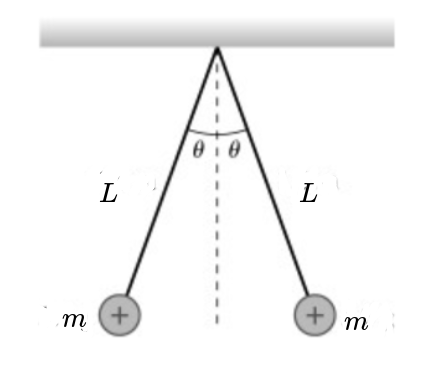
\includegraphics[scale=0.4]{figures/t2p7.png}
    \end{figure}
    
\end{frame}

\begin{frame}{Semana 2 (13/02/2024) - T2P8}
Considere cuatro cargas $q$ negativas fijas en los vértices de un cuadrado de lado $2L$.
Demuestre que si una carga $Q$ positiva de masa $m$ se libera a una pequeña distancia horizontal $\epsilon$ del centro del cuadrado, describirá un movimiento oscilatorio con frecuencia angular $$\omega\sim\sqrt{\frac{k_eqQ}{m}}.$$
\end{frame}